
\documentclass{report}

\input{preamble}
\input{macros}
\input{letterfonts}

\title{\Huge{Algebra Lineare}\\Sistemi Informativi Aziendali}
\author{\huge{Caberlotto Giovanni}}
\date{}

\begin{document}

\maketitle
\newpage% or \cleardoublepage
% \pdfbookmark[<level>]{<title>}{<dest>}
\pdfbookmark[section]{\contentsname}{toc}
\tableofcontents
\pagebreak

\chapter{Matrici} % (fold)
\label{chap:Matrici}

\section{Matrici}

\subsection{Definizione di matrice}

\dfn{Matrice}{Con il termine matrice intendiamo una tabella ordinata di elementi appartenenti allo stesso insieme}
\\
\\
$ 
A=\begin{pmatrix}
  a_{11} & a_{12} & ... & a_{1n} \\
  a_{21} & a_{22} & ... & a_{2n} \\
  \vdots & \vdots & \vdots & \vdots \\
  a_{m1} & a_{m2} & ... & a_{mn} \\
\end{pmatrix}
$
\\
\\
I pedici di ogni elemento della matrice hanno un significato ben preciso: il primo e il secondo numero indicano rispettivamente la riga e la colonna in cui l'elemento è posizionato.
\\
\\
Ogni elemento ha una posizione precisa e, in generale, con la notazione $ a_{ij} $ si indica l'elemento della matrice $ A $ che corrisponde all'incrocio tra la riga i-esima e la colonna j-esima.
\\ 
\\
Un modo alternativo per scrivere una matrice in termini generici, caratterizzandone il numero di colonne ma senza specificarne gli elementi, prevede di indicare il generico elemento $ a_{ij} $ tra parentesi tonde. Nel caso in esame:
\\
\\
$ A = (a{ij})i=1...m, \ j=1...n $
\\
\\
\dfn{Dimensione di una matrice}{Chiamiamo dimensione di una matrice il prodotto tra il numero di righe e il numero di colonne. Tale prodotto va indicato come tale e non come numero: ad esempio se una matrice $A$ ha $m$ righe e $n$ colonne, diciamo che $A$ ha dimensione $m \ x \ n$}
\\
\\
Inoltre, una matrice di dimensione $m \ x \ n$ viene detta matrice di tipo $ (m,n) $, e se i suoi elementi sono numeri reali, si dice che essa appartiene a $\mathbb{R}^{m \ x \ n}$, spesso indicato come $ \mathbb{R}^{m,n} $ oppure come $Mat(m,n,\mathbb{R})$
\\
\\
\dfn{Matrice riga}{Con matrice riga intendiamo una matrice di tipo $ (1,n) $, ossia una matrice formata da una solo riga, indipendentemente dalle colonne}
\\
\\
Le matrici riga vengono usate per riportare le componenti di un vettore, motivo per cui vengono anche dette vettore riga.
\\
\\
$ 
\begin{pmatrix}
-1 & 0 & 2 & 3
\end{pmatrix} \in \mathbb{R}^{1,4} \begin{pmatrix}
  \frac{1}{3} & 2
\end{pmatrix} \in \mathbb{R}^{1,2}
$
\\
\\
\dfn{Matrice colonna}{Una matrice colonna è una matrice formata da una sola colonna, ossia del tipo $ (m,1) $}
\\
\\
Viene anche detta vettore colonna
\\
\\
$ 
\begin{pmatrix}
  -3 \\
  5 \\
  3 \\
  0 \\
  7
\end{pmatrix} \in \mathbb{R}^{5,1}
$
\\
\\
\dfn{Matrice rettangolare}{Con matrice rettangolare intendiamo una matrice in cui il numero delle righe è diverso dal numero delle colonne, cioè con $ m \neq n $}
\\
\\
$  

\begin{pmatrix}
  -1 & 0 & 7 \\
  4 & 6 & -2 
\end{pmatrix} \in \mathbb{R}^{2,3}\begin{pmatrix}
  5 & 8 \\
  3 & -5 \\
  0 & 1 \\
  -1 & 3 
\end{pmatrix} \in \mathbb{R}^{4,2}

$
\\
\\

\dfn{Matrice quadrata}{La matrice quadrata è una matrice che ha il numero di righe uguale al numero di colonne $ (m = n) $, e questo numero pernde il nome di ordine della matrice}
\\
\\
Tali matrici rivestono un ruolo fondamentale in Algebra Lineare. sono infatti le uniche per cui (spoiler!) si può calcolare il determinante e cercare la matrice inversa (se esiste).
\\
\\
$
  \begin{pmatrix}
    -2 & 3 \\
    1 & 1 
  \end{pmatrix} \in \mathbb{R}^{2,2} \ \begin{pmatrix}
    4 & -1 & 2 \\
    0 & 5 & 0 \\
    1 & 2 & -3 
  \end{pmatrix} \in \mathbb{R}^{3,3}
$
\\
\\
esse sono due matrici quadrate, la prima di ordine 2 e la seconda di ordine 3.
\\
\\
In una matrice quadrata si dice:
\\
\begin{itemize}
  \item Diagonale principale, la diagonale che va dall'angolo in alto a sinistra all'angolo in basso a destra;
  \item Digonale secondaria, la diagonale che dall'angolo in alto a destra all'angolo in basso a sinistra.
\end{itemize}
\\
\\
Diagonale principale
\\
$ 
\begin{pmatrix}
  \textcolor{red}{4} & -1 & 2 \\
    0 & \textcolor{red}{5} & 0 \\
    1 & 2 & \textcolor{red}{-3} 

\end{pmatrix}
$
\\
\\
Diagonale secondaria o antidiagonale
\\
$ 
\begin{pmatrix}
  4 & -1 & \textcolor{red}{2} \\
  0 & \textcolor{red}{5} & 0 \\
  \textcolor{red}{1} & 2 & -3 
\end{pmatrix}
$  
\\
\\
\dfn{Matrice diagonale}{è una matrice quadrata in cui gli elementi sono tutti nulli ad eccezzione di quelli sulla diagonale principale}
In formule:
\\
\\
$ A \in \mathbb{R}^{n,m}$ matrice diagonale $ \leftrightarrow \forall i,j \in {1,2,...,n}, i \neq j, a_{ij} = 0$
\\
\\
$  
\begin{pmatrix}
  -1 & 0 & 0 \\
  0 & 2 & 0 \\
  0 & 0 & 3 
\end{pmatrix}
$
\\
\\
\dfn{Matrice antidiagonale}{è una matrice quadrata in cui i soli termini della diagonale secondaria possono essere diversi da zero}

$  
\begin{pmatrix}
  0 & 0 & 7 \\
  0 & 15 & 0 \\
  3 & 0 & 0 
\end{pmatrix}
$
\\
\\
\dfn{Matrice identità}{si indica generalmente con $Id, \ Id_n, \ I$ o con $I_n$ ed è una matrice diagonale avente tutti 1 sulla diagonale principale e tutti 0 altrove}
\\
\\
In simboli:
\\
$Id_n \in \mathbb{R}^{n,m}, \forall i,j \in {1,2,...,n} : a_{ij} = \begin{cases}
  0 \ se \ i \neq j \\
  1 \ se \ i = j \\
\end{cases}$ 
\\
\\
$ 
  \begin{pmatrix}
    1 & 0 & 0 \\
    0 & 1 & 0 \\
    0 & 0 & 1 \\
  \end{pmatrix}
$
\\
\\
Per la moltiplicazioni tra matrice A quadrata generica e matrice Id vale la proprietà comutativa
\\
\\
\dfn{Matrice nulla}{La matrice nulla è una matrice (rettangolare o quadrata) di dimensione qualsiasi, costituita da soli 0 e indicata col simbolo $O$}
\\
\\
\dfn{Matrice triangolare superiore}{La matrice triangolare superiore è una matrice quadrata avente tutti gli elementi al di sotto della diagonale principale uguali a zero}
\\
\\
In formule:
\\
\\
$ A \in \mathbb{R}^{n,m} $ triangolare superiore $ \leftrightarrow \forall i,j \in {1,2,...,n}, i > j : a_{ij} = 0$
\\
\\
\dfn{Matrice triangolare inferiore}{La matrice triangolare inferiore è una matrice quadrata avente tutti gli elementi al di sopra della diagonale prinvipale uguali a 0}
\\
\\
In formule:
\\
\\
$ A \in \mathbb{R}^{n,m} $ triangolare superiore $ \leftrightarrow \forall i,j \in {1,2,...,n}, i < j : a_{ij} = 0$
\\
\\
\dfn{Matrici a scalini}{Una qualsiasi matrice (quadrata o rettangolare) è detta matrice a scalini o matrice a gradini se il primo elemento diverso da zero della $i$-esima riga, con $i > 1$, è più a destra del primo elemento diverso da zero della riga precedente}
\\
\\
$
\begin{pmatrix}
  1 & 2 & 1 \\
  0 & 1 & 2 \\
  0 & 0 & 3 
\end{pmatrix}
\begin{pmatrix}
  1 & 2 & 0 & 1 \\
  0 & 2 & 1 & 0 \\
  0 & 0 & 1 & 3
\end{pmatrix}
$
\\
\\
Le matrici appena elencate sono matrici a scalini mentre non lo è la matrice:
\\ 
$ 
\begin{pmatrix}
  5 & 0 & 3 & 8 \\
  0 & 2 & 0 & 0 \\
  0 & 9 & 2 & 6 
\end{pmatrix}
$
\\
\\
Il primo elemento diverso da zero su ogni riga (quando c'è) è detto pivot.
\\
\\
(spoiler!) tramite il metodo di eliminazione di Gauss è possibile ridurre qualsiasi matrice in una matrice a scalini
\\
\\
\dfn{Matrice simmetrica e matrice antisimmetrica}{Una matrice quadrata di ordine n > 1 si dice simmetrica se i suoi elementi sono simmetrici rispetto alla diagonale principale}
\\
\\
ossia per ogni:
\\
\\
$ i,j \in {1,2,...,n}, con \ i \neq j : a_{ij} = a_{ji}$
\\
\\
di contro una matrice è detta assimetrica se $a_{ij} = -a_{ji}$ 

\subsection{Operazioni fra matrici}

\subsubsection{Somma fra matrici}

L'operazione di addizione tra matrici può essere eseguita solo se le matrici sono dello stesso tipo: $A_{ij},B_{ij}, ij = ij$
\\
\\
\dfn{Somma tra matrici}{La somma di due matrici dello stesso tipo di ordine $(m \ x \ n)$ è la matrice ancora di ordine $(m \ x \ n)$ che ha come elementi la somma delle coppie di elementi che occupano la stessa posizione nelle due matrici addendi}
Cioè:
\\
\\
Date $A_{ij} \in \mathbb{R}$ e $B_{ij} \in \mathbb{R}$ 
\\
\\
la somma tra le due matrici genererà la matrice C:
\\
\\
$
C = \begin{pmatrix}
  a_{11} + b_{11} & a_{12} + b_{12} & a_{1n} + b_{1n} \\
  a_{21} + b_{21} & a_{22} + b_{22} & a_{2n} + b_{2n} \\
  ... & ... & ... \\
  a_{m1} + b_{m1} & a_{m2} + b_{m2} & a_{mn} + b_{mn} \\

\end{pmatrix}
$
\\
\\
$aTe = eTa$ Operatore di operazione generica
\\
\\
L'elemento neutro della somma fra matrici è la matrice nulla
\\
\\
$(A_{ij} \in \mathbb{R}) + (O_{ij} \forall i,j = 0) = A$
\\
\\
La somma fra la matrice $A_{ij} \in \mathbb{R}$ e la matrice opposta $-A_{ij} \in \mathbb{R}$ è uguale alla matrice nulla
\\
\\
$
A + (-A) = O
$
\subsubsection{Prodotto di una matrice per uno scalare}

\dfn{Prodotto di una matrice per uno scalare}{Dato un numero reale $\lambda$ e una matrice $A^{(m \ x \ n)}$, il prodotto del numero $\lambda$ per la matrice $A$ è una matrice i cui elementi si ottengono dagli elementi di $A$ moltiplicati per il numero $\lambda$}
\\
\\
$
\lambda * A = \begin{pmatrix}
  \lambda a_{11} & \lambda a_{12} & \lambda a_{1n}  \\
  \lambda a_{21}  & \lambda  a_{22}  & \lambda a_{2n}  \\
  ... & ... & ... \\
  \lambda a_{m1}  & \lambda a_{m2}  & \lambda a_{mn}  \\
\end{pmatrix}
$
\subsubsection{Prodotto fra matrici}

Il prodotto fra matrici può essere fatto solo se il numero delle colonne della matrice $A$ è uguale al numero di righe della matrice $B$

\dfn{Prodotto fra matrici}{Date due matrici tali che il numero di colonne della matrice $A$ sia uguale al numero di righe della matrice $B$, ogni elemento $c_{ij}$ della matrice prodotto $C$ è uguale alla somma dei prodotti degli elementi della riga $i-esima$ dellamatrice $A^{m,n}$ per gli elementi corrispondenti della colonna $j-iesima$ della matrice $B^{m,p}$ la matrice risultante sarà la matrice $C$^{m,p}}



\subsubsection{Proprietà del prodotto fra matrici}

\begin{itemize}
  \item Non gode della proprietà comutativa;
  \item Proprietà associativa;
  \item Proprietà distritibutiva;
  \item Elemento neutro matrice identità;
  \item Moltiplicando una qualsiasi matrice $M$ per la matrice nulla $O$, nell'ipotesi in cui il prodotto sia eseguibile, si ottiene la matrice nulla $O$
  \item Non vale la legge di annullamento del prodotto.
\end{itemize}

\subsubsection{Il prodotto tra matrici in formule}

Siano $A$ e $B$ due matrici a elementi appartenenti in un campo $\mathbb{K}$ tali che il numero di colonne di $A$ sia uguale al numero di righe di $B$, cioè:
\\
\\
$A \in \ Mat(m,n,\mathbb{K}), \ B \in \ Mat(n,p,\mathbb{K})$
\\
\\
Esprimiamo gli elementi di ciascuna matrice in forma compatta:
\\
\\
$A=(a_{ij})
\\
1 \le i \le m \\
1 \le j \le n 
$
\\
\\
$B=(b_{ij})
\\
1 \le i \le n \\
1 \le j \le p 
$
\\
\\
e chiamiamo $C = (c_{ij}) \in \ Mat(m,p,\mathbb{K})$ la matrice prodotto tra $A$ e $B$ 
\\
Gli elementi di $C=AB$ si ottengono dalla seguente formula
\\
\\
$c_{ij} = \sum_{k=1}^{n} a_{ik}b_{kj}, \forall i \in {1,2,...,m}, \forall j \in {1,2,...,p}$

\subsection{Eliminazione Gaussiana}

L'eliminazione gaussiana, chamata anche metodo di eliminazione di Gauss e spesso abbreviata con l'acronimo MEG, prende il nome dal matematico tedesco Carl Friedrich Gauss ed è un algoritmo che consente di risurre qualsiasi matrice in una matrice a scalini con quello che viene detto algoritmo di Gauss.
Il metodo di risoluzione gaussiana è tra i più utilizzati in Algebra Lineare ed è usato per risolvere i sistemi lineari e per calcolare il rango di una matrice. Inoltre, una sua variante, detta metodo di eliminazione di Gauss-Jordan, permette di calcolare la matrice inversa di ogni matrice quadrata invertibile.
\\
\\
Consideriamo una qualsiasi matrice a componenti reali $A \in \mathbb{R}^{m,n}$ e indichiamo con $R_1,R_2,...,R_m$ le sue righe:
\\
\\


  $ 
    A = \begin{pmatrix}
      a_{11} & a_{12} & ... & a_{1n} \\
      a_{21} & a_{22} & ... & a_{2n} \\
      a_{i1} & a_{i2} & ... & a_{in} \\
      a_{m1} & a_{m2} & ... & a_{mn} \\
    \end{pmatrix} \rightarrow \begin{cases}
      \rightarrow \ prima \ riga \ R_1 \\
      \rightarrow \ seconda \ riga \ R_2 \\
      \rightarrow \ i-esima \ riga \ R_i \\
      \rightarrow \ m-esima \ riga \ R_m \\
    \end{cases}
  $ 
\\
\\
L'intento del metodo di eliminazione di Gauss è di ridurre la matrice generica in una matrice a scalini, e per farlo possiamo utilizzare quelle che si chiamano mosse di Gauss
\\
\\
\begin{enumerate}
  \item{Si $C_k$, con $1 \le k \le n$, la prima colonna a partire da sinistra contiene almeno un termine $a$ non nullo.
  \\
  Detta $R_1$ la prima riga della matrice, possono presentarsi due eventualità:}
  \item{
    \begin{itemize}
      \item se $a$ è un elemento di $R_1$, passiamo al punto 3;
      \item se $a \not\in R_1$, scambiamo la riga che contiene $a$ con $R_1$. Controlliamo se la matrice ottenuta dopo lo scambio è ridotta a gradini: se lo è possiamo fermarci, in caso contrario procediamo oltre.
    \end{itemize}
    }
  \item{
      L'obiettivo è annullare tutti gli elementi della $k-esima$ colonna al di sotto di $a$. Sostituiamo ogni riga $R_i$, con $i > 1$ e con $k-esimo$ elemento non nullo, con $R_i + \lambda R_1$. Qui $\lambda$ è uno scalare scelto in maniera tale che la somma tra $R_i$ e $\lambda R_1$ abbia il $k-esimo$ elemeno nullo.
    }
  \item{
      Se la matrice risultante è ridotta a scalini, l'algoritmo è terminato. in caso contrario ripetiamo l'algoritmo in modo ricorsivo fino al raggiungimento del risultato ottenuto.
    }
\end{enumerate}

\\
\\

\nt{Il risultato dell'algoritmo non è sempre lo stesso, ma dipende dalle scelte effettuate}

\subsubsection{Esempio di applicazione del metodo di eliminazione di Gauss}

\ex{Riduzione matrice generica in matrice a scalini con metodo di eliminazione di Gauss}{
Sia data la matrice:
\\
$  
A = \begin{pmatrix}
  0 & 0 & 1 & -1 \\
  0 & 1 & 3 & 0 \\
  0 & 2 & 1 & 5 
\end{pmatrix}
$

La prima colonna non nulla a partire da sinistra è $C_2$, quindi tralasciamo $C_1$.
\\
Il primo elemento di $C_2$ è zero, per cui sostituiamo la prima riga con una a scelta tra la seconda e la terza: 
\\
in questo esempio prendiamo la seconda e la scambiamo con la prima
\\
$  
A' = \begin{pmatrix}
  0 & 1 & 3 & 0 \\
  0 & 0 & 1 & -1 \\
  0 & 2 & 1 & 5 
\end{pmatrix}
$
\\
L'elemento $a'_{12}$ è diverso da zero e dobbiamo annullare gli elementi sottostanti.
\\
$a'_{22} = 0$, quindi la seconda riga rimane così com'è, mentre $a'_{32} = 2$. per annullarlo moltiplichiamo la prima riga per $-2$ e la sommiamo alla terza:
\\
\\
$-2R_1 + R_3 = -2\begin{pmatrix}0 & 1 & 3 & 0\end{pmatrix} + \begin{pmatrix}0 & 2 & 1 & 5\end{pmatrix} = \begin{pmatrix}0 & -2 & -6 & -0\end{pmatrix} + \begin{pmatrix}0 & 2 & 1 & 5\end{pmatrix} = \begin{pmatrix}0 & 0 & -5 & 5\end{pmatrix}$
\\
\\
Sostituiamo $R_3 \rightarrow -2R_1 + R_3$
\\
ottenendo la matrice
\\
$  
A'' = \begin{pmatrix}
  0 & 1 & 3 & 0 \\
  0 & 0 & 1 & -1 \\
  0 & 0 & -5 & 5 
\end{pmatrix}
$
\\
Concludiamo con la sostizione:
\\
$R_3 \rightarrow 5R_2 + R_3$
\\
il risultato è la matrice
\\
$  
A'''=\begin{pmatrix}
  0 & 1 & 3 & 0 \\
  0 & 0 & 1 & -1 \\
  0 & 0 & 0 & 0 
\end{pmatrix}
$
\\ 
la quale è una matrice a scalini i cui pivot sono: $a'''_{12} = 1, a'''_{23} = 1$.
}
\subsection{Determinante di una matrice}
Il determinante di una matrice è un numero associato a ciascuna matrice quadrata, e ne esprime alcune proprietà algebriche e geometriche. Se $A$ è una matrice quadrata, il suo determinante si indica con $det(A)$, o più raramente con $|A|$, e si calcola in modi differenti a seconda della dimensione della matrice.

\nt{Il caloclo del determinante è definito solo per matrici quadrate, non è possibile quindi calcolare il determinante di una matrice rettangolare}

\subsubsection{Determinante di matrici 2x2}
Il determinante di una matrice quadrata di ordine 2 è dato dal prodotto degli elementi della diagonale principale meno il prodotto degli elementi dell'antidiagonale.
\\
Dunque data una matrice 2x2 possiamo calcolare il determinante con la seguente formula:
\\
\\ 
$det\begin{pmatrix}
  a & b \\
  c & d
\end{pmatrix} = (a * d) - (b * c)$
\\
\\
Il determinante di una matrice formata da un solo elemento è uguale all'elemento stesso:
\\
\\
det(a_{11})=a_{11}

\subsubsection{Esempi sul determinante di una matrice di ordine 2}
\ex{Calcolo determinante matrici 2x2}{Date le seguenti matrici calcolane il determinante
\\
$A = \begin{pmatrix}
  1 & 3 \\
  4 & 5 
\end{pmatrix}
B = \begin{pmatrix}
  6 & 12 \\
  3 & 6 
\end{pmatrix}
C = \begin{pmatrix}
  -2 & 5 \\
  0 & -1
\end{pmatrix}
$
\\
Applichiamo la formula per il calcolo del determinante a ciascuna matrice
\\
$  
det(A) = det \begin{pmatrix}
  1 & 3 \\
  4 & 5 
\end{pmatrix} = (1 * 5) - (3 * 4) = 5 - 12 = -7 \\
det(B) = det \begin{pmatrix}
  6 & 12 \\
  3 & 6 
\end{pmatrix} = (6 * 6) - (12 * 3) = 36 - 36 = 0 \\
det(C) = det \begin{pmatrix}
-2 & 5 \\
  0 & -1 
\end{pmatrix} = (-2 * (-1)) - (5 * 0) = 2 - 0 = 2
$

}

\subsubsection{Determinante di matrici 3x3 con la regola di Sarrus}
Per calcolare il determinante di una matrice quadrata di ordine 3 possiamo applicare la regola di Sarrus, secondo cui:
\\
$ det \begin{pmatrix}
  a_{11} & a_{12} & a_{13} \\
  a_{21} & a_{22} & a_{23} \\
  a_{31} & a_{32} & a_{33} 
\end{pmatrix} = (a_{11}*a_{22}*a_{33}+a_{12}*a_{23}*a_{31}+a_{13}*a_{21}*a_{32})-(a_{13}*a_{22}*a_{31}+a_{12}*a_{21}*a_{33}+a_{11}*a_{23}*a_{32})$

Ricordarla a memoria sarebbe quasi impossibile. per fortuna esiste un modo comodo che permette di ricavarla: basta riscrivere la matrice accostando la matrice stessa sulla sua destra per poi:
\begin{enumerate}
  \item Sommare i prodotti lungo le prime tre diagonali complete da sinistra verso destra;
  \item Sommare i prodotti lungo le ultime tre antidiagonali complete percorse da destra verso sinistra;
  \item Calcolare la differenza tra i risultati ottenuti.
\end{enumerate}
\\
Graficamente l'operazione risulta essere la seguente:
\\

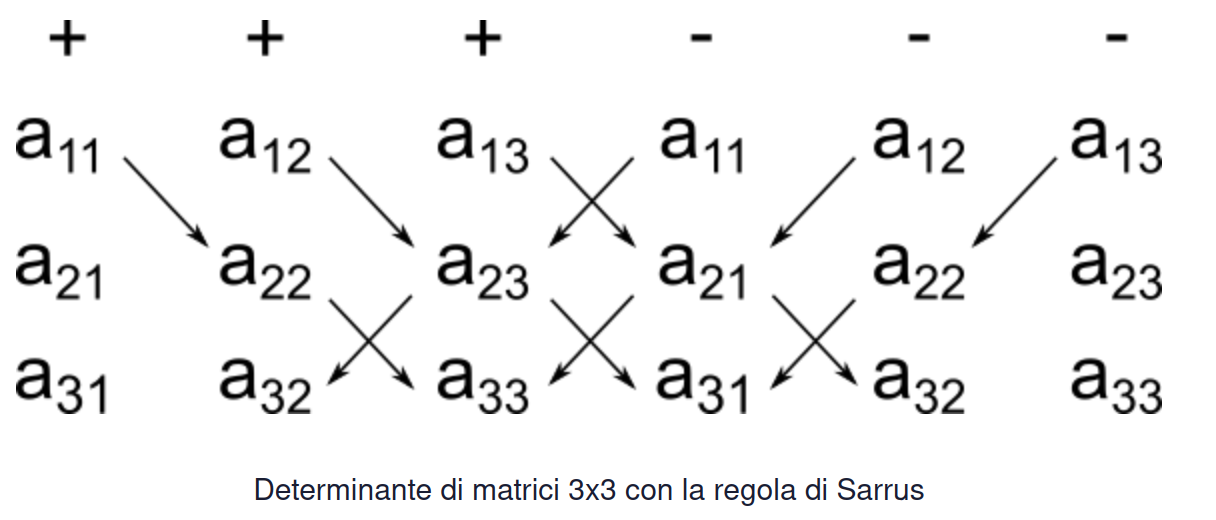
\includegraphics[width=0.6\textwidth]{./graphs/sarrusGraph/sarrusGraph.png}

\subsubsection{Esempio di applicazione della regola di Sarrus}

\ex{Calcolo del determinante applicando Sarrus}{
Calcola il determinante della matrice $A$ applicando la regola di Sarrus
\\
$A=\begin{pmatrix}
  2 & -1 & 4 \\
  1 & 2 & 0 \\
  3 & 5 & 1
\end{pmatrix}
$
\\
\\
Scriviamo due matrici l'una accanto all'altra e senza parentesi e tracciamo le tre diagonali complete procedendo da sinistra verso destra e le tre antidiagonali procedendo da destra verso sinistra.
\\
\\
$  
\begin{pmatrix}
2 & -1 & 4 & 2 & -1 & 4 \\
1 & 2 & 0 & 1 & 2 & 0 \\
3 & 5 & 1 & 3 & 5 & 1  
\end{pmatrix}$
\\
\\
(Per comodita di formattazione sono state aggiunte le parentesi)
\\
Sommiamo i prodotti lungo le prime tre diagonali principali
\\
\\
$(2*2*1)+(-1*0*3)+(4*1*5) = 24$
\\
\\
Ora sommiamo i prodotti delle ultime tre antidiagonali
\\
\\
$(4*2*3)+(-1*1*1)+(2*0*5) = 23$
\\
\\
Sottraendo, nell'ordine i due risultati otteniamo il determinante della matrice $A$:
\\
\\
$det(A) = 1$
}

\subsubsection{Determinante di matrici quadrate di qualsiasi ordine col teorema di Laplace}

Il teorema di Laplace permette di calcolare il determinante di una matrice quadrata attraverso formule ricorsive, dette sviluppi di Laplace, che possono essere applicate per righe o per colonne, e che si possono applicare a matrici quadrate di ordine qualsiasi (anche a matrici 2x2 o 3x3)
\\
\\
Consideriamo una matrice quadrata di ordine $n$
\\
\\
$A = \begin{pmatrix}
  a_{11} & a_{12} & ... & a_{1n} \\
  a_{21} & a_{22} & ... & a_{2n} \\
  ... & ... & ... & ... \\
  a_{m1} & a_{m2} & ... & a_{mn}
\end{pmatrix}
$
\\
\\
e denotiamo con $A_{ij}$ la matrice che si ottiene eliminando la riga $i$ e la colonna $j$ del suo determinante.
\\
\\
Fissato un qualsiasi elemento $a_ij \in A$, chiamiamo complemento algebrico (o cofattore) di $a_{ij}$ il numero:
\\
\\
$(-1)^{i+j} * det(A)$
\\
\\
Sviluppo di Laplace per righe 
\\
\\
Fissata una qualsiasi riga della matrice $A$, il determinante di $A$ è pari alla somma dei prodotti degli elementi della riga scelta per i rispettivi complementi algebrici. In formule:
\\
\\
$det(A) = \sum_{j=1}^{n} [a_{ij}*(-1)^{i+j}*det(A_{ij})$
\\
\\
\nt{Ci si muove lungo la i-esima riga}
\\
\\
Sviluppo di Laplace per colonne
\\
\\
Fissata una qualsiasii colonna di $A$, il suo determinante è uguale alla somma dei prodotti degli elementi della colonna fissata per i rispettivi complementi algebrici. In formule:
\\
\\
$det(A) = \sum_{i=1}^{n} [a_{ij}*(-1)^{i+j}*det(A_{ij})$
\\
\\
\nt{ci si muove lungo la j-esima colonna}

\subsubsection{Esempio di applicazione del teorema di Laplace per il calcolo del determinante}

\ex{Calcolo del determinante applicando il teorema di Laplace}{
Data la matrice $A$ calcola il determinante applicando Laplace
\\
\\
$  
A = \begin{pmatrix}
  1 & 0 & 5 \\
  2 & -1 & 0 \\
  7 & -2 & 0 
\end{pmatrix}
$
\\
\\
Tra tutte le colonne e tutte le righe di $A$ vediamo subito che la terza colonna contiene due zeri, quindi decidiamo di calcolare il determinante con uno sviluppo per colonna scegliendo proprio la terza colonna.
\\
\\
Dobbiamo sommare i prodotti degli elementi della terza colonna per i rispettivi complementi algebrici. Se un elemento è 0, il prodotto per il suo complemento algebrico dà 0, quindi basta considerare solo gli elementi non nulli cioè:
\\
\\
$a_{13} = 5$
\\
\\
Il cui complemento algebrico è:
\\
\\
$(-1)^{1+3} * det(A_{13}) = (-1)^4 * det \begin{pmatrix}
  2 & -1 \\
  7 & -2
\end{pmatrix} \\
= 1 * [(2*(-2))-(-1*7)] = 3$
\\
\\
Dunque:
\\
\\
$det(A) = 5 * 3 = 15$
}

\subsubsection{Proprietà del determinante}
Vediamo ora le principali proprietà del determinante che, oltre a rivestire un importante ruolo teorico, ci permettono di risparmiare un bel pò di tempo quando dobbiamo fare i calcoli.
\\
\\
Determinante nullo: il determinante di una matrice quadrata è uguale a 0 se e solo se
\begin{itemize}
  \item Ha una riga (o una colonna) tutti di elementi nulli;
  \item Due righe (o due colonne) sono proporzionali;
  \item Una riga (o una colonna) è una combinazioni lineare di due o più righe (o colonne).
\end{itemize}
\\
\\
Determinante di matrici triangolari: se la matrice quadrata di cui vogliamo calcolare il determinante è una matrice triangolare (superiore o inferiore), allora il determinante è dato dal prodotto degli elementi della diagonale principale.
\\
\\
Determinante del prodotto: se siamo di fronte a due matrici quadrate dello stesso ordine, tra le quali è quindi possibile eseguire il prodotto riga per colonna, il determinante del prodotto è uguale al prodotto dei determinanti:
\\
\\
$det(AB) = det(A)*det(B)$
\\
\\
Tale proprietà in realtà è un vero e proprio teorema conosciuto con il nome di teorema di Binet.
\\
\\
Determinante dell'inversa: data una matrice invertibile, il determinante della matrice inversa è il reciproco del determinante della matrice di partenza
\\
\\
$det(A^{-1}) = \frac{1}{det(A)}$
\\
\\
Determinante della trasposta: una matrice quadrata e la sua matrice trasposta hanno lo stesso determinante
\\
\\
$ det(A^{T}) = det(A)$
\\
\\
Determinante del prodotto per uno scalare: il determinante del prodotto di una matrice per uno scalare è dato dal prodotto tra lo scalare elevato all'ordine della matrice e il determinante della matrice; dunque se $A$ è una matrice quadrata di ordine $n$ e $\lambda$ è lo scalare abbiamo che:
\\
\\
$det(\lambda A) = \lambda^n * det(A)$
\\
\\
Determinante di matrici simili: due matrici simili hanno lo stesso determinante

\subsection{Sottomatrice e minori di una matrice}

Data una qualsiasi matrice, prendono il nome di sottomatrici quelle matrici ottenute eliminando alcune righe e/o colonne della matrice in esame, mentre si dicono minori associati a una matrice i determinanti delle sottomatrici quadrate da essa estratte

\subsubsection{Sotomatrice}
Sia $A$ una matrice qualsiasi con $m \ge 1$ righe e $n \ge 1$ colonne. Si dicono sottomatrici di $A$ tutte quelle matrici estratte da $A$ eliminando un numero arbitrario di righe e/o di colonne.
\\
\\
In alternativa, possiamo definire sottomatrice di $A$ qualsiasi matrice costruita prendendo gli elementi dell'intersezione di $r$ righe e $s$ colonne di $A$, con $0 \le r \le m$, e $0 \le s \le n$

\ex{Esempi di sottomatrice}{Consideriamo la matrice 
\\
\\
$  
  A = \begin{pmatrix}
    1 & 0 & 2 & 4 \\
    5 & 7 & 6 & 8 \\
    -2 & 3 & -1 & 9 
  \end{pmatrix}
$
\\
\\
Sono sottomatrici di $A$:
\\
\\
$  
A' = \begin{pmatrix}
  1 & 0 & 2 \\
  5 & 7 & 6 \\
  -2 & 3 & -1
\end{pmatrix}
$
\\
\\
La quale è stata ottenuta eliminando l'ultima colonna di $A$ o, equivalmente, pensata come l'intersezione tra le sue prime tre righe e tre colonne
\\
\\
$  
A'' = \begin{pmatrix}
  0 & 2 \\
  3 & 1
\end{pmatrix}
$
\\
\\
Ottenuta eliminando la prima e quarda colonna e seconda riga di $A$ o, equivalmente, ricavata come intersezione tra prima e terza riga e seconda e terza colonna di $A$.
\\
\\
$ 
A''' = \begin{pmatrix}
  7 & 8
\end{pmatrix}
$
\\
\\
estratta eliminando prima e terza riga e prima e terza colonna di $A$
}

\subsubsection{Minori di una matrici}

Dopo aver introdotto il concetto di sottomatrice possiamo dare la definizione di minore di una matrice, partendo da quella generale per poi passare in rassegna, uno per per volta, i vari tipi di minori, fornendone la definizione e qualche esempio.
\\
\\
Potrebbe sembrare un inutile elenco di nozioni teoriche, ma non sottovalutarle! Ribadiamo ancora una volta che i concetti che vedremo sono strumenti utili a calcolare il rango, a studiare la definitezza di una matrice, a risolvere i sistemi lineari e a calcolare la matrice inversa, ed è bene quindi capire come si definiscono e, soprattutto, come si costruiscono.
\\
\\
Consideriamo una qualsiasi matrice $A$ (quadrata o rettangolare) con $m \ge 1$ righe e $n \ge 1$ colonne
\\
\\
Si definisce minore della matrice $A$ il determinante di una sottomatrice quadrata di $A$; l'ordine della sottomatrice è detto ordine del minore.
\\
\\
In alcune situazioni con minore di una matrice si intende, semplicemente, una sottomatrice quadrata di una data matrice, ma niente paura: sarà il contesto a far capire se ci si sta riferendo al minore come determinante o al minore come sottomatrice.
\\
\\
\subsubsection{Esempi sui minori di una matrice}
\ex{Esempi di minori di una matrici}{Prendiamo in esame la seguente matrice:
\\
\\
$
A = \begin{pmatrix}
  2 & 1 & 4 \\
  -1 & 0 & -2 \\
  3 & 6 & 5 \\
  -4 & 7 & -3 
\end{pmatrix}
$
\\
\\
I minori di ordine 3 sono:
\\
\\
$det \begin{pmatrix}
  -1 & 0 & 2 \\
  3 & 6 & 5 \\
  -4 & 7 & -3 
\end{pmatrix} = 37 \ ; \ det \begin{pmatrix}
  2 & 1 & 4 \\
  3 & 6 & 5 \\
  -4 & 7 & -3 
\end{pmatrix} = 63 
\\
\\
det \begin{pmatrix}
  2 & 1 & 4 \\
  -1 & 0 & 2 \\
  -4 & 7 & -3 
\end{pmatrix} = 5 \ ; \ det \begin{pmatrix}
  2 & 1 & 4 \\
  -1 & 0 & 2 \\
  3 & 6 & 5 
\end{pmatrix} = 1
$
Ottenuti calcolando i determinanti delle sotto matrici ricavate eliminando, rispettivamente, prima, seconda, terza e quarta riga di $A$
\\
\\
L'operazione può essere esiguita calcolando i minori di ordine 2 ecc.
}

\subsection{Matrice inversa}
La matrice inversa può essere calcolata solo per le matrici quadrate invertibili ed è quella matrice che, moltiplicata per la matrice di partenza, restituisce la matrice identità.

\subsubsection{Definizione di matrice inversa}
\dfn{Matrice inversa}{Una matrice quadrata $A$ di ordine $n$ è detta matrice invertibile se esiste una matrice quadrata dello stesso ordine della matrice $A$, solitamente indicata con $A^{-1}$, tale che il prodotto riga per colonna tra le due matrici restituisce la matrice identità di ordine $n$}
\\
\\
In formule:
\\
\\
$A$ matrice quadrata invertibile $\leftrightarrow \exist A^{-1}$ tale che $A*A^{-1} = Id_n = A^{-1}*A$
\\
\\
Da notare che tale definizione ci suggerisce un modo per verificare se la matrice ottenuta è effettivamente l'inversa della matrice di partenza. Dopo aver determinato la presunta matrice inversa basta, infatti, calcolare il prodotto $A*A^{-1}$: se esso coincide con la matrice identità allora è tutto ok, se non è così è stato sbagliato qualche procedimento del algoritmo.
\\
\\
Se, come succede nella stragrande maggioranza dei casi, $A$ è una matrice quadrata a coefficienti in un campo $\mathbb{K}$ (ad esempio nel campo $\mathbb{R}$ dei numeri reali o nel campo $\mathbb{C}$ dei numeri complessi) allora $A$ è invertibile se e solo se il suo determinante è diverso da zero.
\\
\\
$A \in Mat(m,n,\mathbb{K})$ matrice quadrata invertibile $\leftrightarrow det(A) \neq 0$

\subsubsection{Come calcolare la matrice inversa di una matrice invertibile}

Sia $A$ una matrice quadrata a coefficienti in un campo $\mathbb{K}$, cioè $A \in Mat(m,n,\mathbb{K})$
\\
\\
La prima cosa da fare è stabilire se si tratta di una matrice invertibile, ossia stabilire se il determinante di $A$ è diverso da zero.
\\
\\
Dunque, per calcolare la matrice inversa dobbiamo:
\\
\begin{enumerate}
  \item{Calcolare il determinante di A:
      \begin{itemize}
        \item Se $det(A) = 0$: Niente da fare zi! la matrice non è invertibile;
        \item Se $det(A) \neq 0$: allora l'inversa esiste e possiamo proseguire;
      \end{itemize}
    }
  \item Calcolare la matrice dei cofattori (o matrice dei complementi algebrici) cioè sostituire ogni elemento della matrice di partenza con il relativo cofattore 
  \item Determinare la matrice trasposta della matrice dei cofattori ottenuta al punto 2, cioè scambiarne le righe con le colonne. (La matrice trasposta della matrice dei cofattori viene anche definita matrice aggiunta)
  \item Moltiplicare la matrice ottenuta al punto 3, per lo scalare $\frac{1}{det(A)}$
  \item Quella del punto 4 è la matrice inversa della matrice di partenza
\end{enumerate}
\\
\\
In sintesi: data una matrica quadrata a coefficienti in un campo $\mathbb{K}$ 
\\
\\
$
A=\begin{pmatrix}
  a_{11} & a_{12} & ... & a_{1n} \\
  a_{21} & a_{22} & ... & a_{2n} \\
  ... & ... & ... & ... \\
  a_{m1} & a_{m2} & ... & a_{mn}
\end{pmatrix}
$
\\
\\
e assunto che la matrice sia invertibile, cioè verificato che $det(A) \neq 0$, la sua matrice inversa è: 
\\
\\
$
A^{-1}=\frac{1}{det(A)}\begin{pmatrix}
  Cof(a_{11}) & Cof(a_{12}) & ... & Cof(a_{1n}) \\
  Cof(a_{21}) & Cof(a_{22}) & ... & Cof(a_{2n}) \\
  ... & ... & ... & ... \\
  Cof(a_{m1}) & Cof(a_{m2}) & ... & Cof(a_{mn})
\end{pmatrix}
$

\subsubsection{Esempio sul calcolo della matrice inversa}

\ex{Esempio sul calcolo della matrice inversa}{
  A titolo di esempio calcoliamo, se esiste, l'inversa della matrice:

  $  
    A = \begin{pmatrix}
      1 & 0 & 1 \\
      2 & -1 & 3 \\
      1 & 4 & 2
    \end{pmatrix}
  $
\\
\\
Cominciamo col calcolo del determinante. 
\\
\\
$ 
det(A) = \begin{pmatrix}
  1 & 0 & 1 \\
  2 & -1 & 3 \\
  1 & 4 & 2 
\end{pmatrix} = 1\cdot\left(-1\right)^{\left(1+1\right)}\cdot\left(\left(-1\cdot2\right)-\left(3\cdot4\right)\right)+\left(1\cdot(-1)^{\left(3+1\right)}\cdot\left((2\cdot4)-(-1)\right)\right)=-5 \neq 0
$
\\
\\
Dunque la matrice è invertibile.
\\
\\
Calcoliamo ora i cofattori dei sui elementi
\\
\\
$ 
Cof(a_{ij}) = (-1)^{nm} * C_{nm}
\\
\\
Cof(a_{11}) = -14 
\\
Cof(a_{12}) = -1
\\
Cof(a_{13}) = 9
\\
Cof(a_{21}) = 4
\\
Cof(a_{22}) = 1
\\
Cof(a_{23}) = -4
\\
Cof(a_{31}) = 1
\\
Cof(a_{32}) = -1
\\
Cof(a_{33}) = -1
$
\\
\\
Formiamo la matrice dei complementi algebrici sostituendo ogni elemento di $A$ col relativo cofattore
\\
\\
$  
\begin{pmatrix}
  -14 & -1 & 9 \\
  4 & 1 & -4 \\
  1 & -1 & -1 
\end{pmatrix}
$
\\
\\
Scriviamone la trasposta
\\
\\
$  
\begin{pmatrix}
  -14 & -1 & 9 \\
  4 & 1 & -4 \\
  1 & -1 & -1 
\end{pmatrix}^T = \begin{pmatrix}
  -14 & 4 & 1 \\
  -1 & 1 & -1 \\
  9 & -4 & -1 
\end{pmatrix}
$
\\
\\
Moltiplicandola per il reciprico del determinante di $A$ otteniamo la matrice inversa cercata
\\
\\
$  
A^{-1} = \frac{1}{-5} * \begin{pmatrix}
  -14 & 4 & 1 \\
  -1 & 1 & -1 \\
  9 & -4 & -1 
\end{pmatrix}
= \begin{pmatrix}
  \frac{14}{5} & \frac{-4}{5} & \frac{-1}{5} \\
  \frac{1}{5} & \frac{-1}{5} & \frac{1}{5} \\
  \frac{-9}{5} & \frac{4}{5} & \frac{1}{5} 
\end{pmatrix}

$
}

\subsubsection{Calcolare la matrice inversa col metodo di Gauss-Jordan}

\subsubsection{Proprietà della matrice inversa}

\begin{enumerate}
  \item L'inversa di una matrice invertibile è una matrice invertibile, e l'inversa dell'inversa coincide con la matrice di partenza:
    \\ 
    \\
    $(A^{-1}^{-1}) = A$
  \item L'inversa del prodotto tra due matrici invertibili è uguale al prodotto tra l'inversa della seconda e l'inversa della prima:
    \\
    \\
    $(AB)^{-1} = B^{-1} * A^{-1} $
  \item Il determinante dell'inversa di una matrice invertibile è il reciproco del determinante della matrice di partenza:
    \\
    \\
    $det(A^{-1}) = \frac{1}{det(A)}$
  \item L'insieme delle matrici quadrate e invertibili di ordine $n$ dotato del prodotto riga per colonna forma un gruppo, il cosiddetto gruppo lineare
\end{enumerate}


\subsection{Rango di una matrice}

Il rango di una matrice, detto anche caratteristica, esprime una proprietà delle matrici che è fondamentale nello studio dell'Algebra Lineare, nella risoluzione di sistemi lineari e nel contesto delle applicazioni lineari.

\subsubsection{Definizione di rango di una matrice}
Sia $A$ una qualsiasi matrice quadrata o rettangolare, a coefficienti in un campo $\mathbb{K}$ (come ad esempio $\mathbb{R}$ o $\mathbb{C})$, con $m$ righe e $n$ colonne. Il suo rango (o caratteristica) si può indicare in uno dei seguenti modi:
\\
\\
$ rango(A), \ rk(A), \ rank(A), \ rg(A), \ p(A), \ r(A) $ 
\\
\\
e altro non è se non un numero intero non negativo associato alla matrice $A$
\\
\\
Si possono dare le seguenti definizioni di rango:
\\
\begin{itemize}
  \item il massimo numero di righe linearmente indipendenti di $A$;
  \item il massimo numero di colonne linearmente indipendenti di $A$;
  \item{ la dimensione dell'immagine dell'applicazione lineare
  \\
  \\
  $ L_A : \mathbb{K}^n \rightarrow \mathbb{K}^m $
  \\
  $ L_A(x) = Ax $}
  \item L'ordine massimo dei minori non nulli che si possono estrarre da $A$, cioè l'ordine massimo delle due sottomatrici quadrate che si possono estrarre da $A$ con determinante diverso da zero;
  \item Il numero di pivot di una riduzione a scala della matrice $A$ attraverso il metodo di eliminazione gaussiana;
  \item La dimensione del sottospazio vettoriale generato dalle righe (o dalle colonne) di $A$
\end{itemize}

\subsubsection{Calcolo del rango di una matrice}
Sia $A$ una matrice con $m$ righe ed $n$ colonne.
\\
\\
Abbiamo definito il rango di $A$ come l'ordine massimo dei minori non nulli che si possono estrarre da $A$. in modo equivalente, il rango di una matrice è l'ordine massimo delle sottomatrici quadrate con determinante diverso da zero che si possono estrarre da $A$
\\
\\
Tale definizione fornisce un metodo per il calcolo del rango, detto criterio dei minori
\\
\\
\begin{enumerate}
  \item{ Consideriamo il minimo tra il numero di righe e il numero di colonne di $A$, ossia $j_1 = min(m,n)$ estraiamo tutte le sottomatrici quadrate $A$ di ordine $j_1$
  \begin{itemize}
    \item Se c'è almeno una sottomatrice quadrata di ordine $j_1$ con determinante diverso da zero, allora $rk(A) = j_1$
    \item Se tutte le sottomatrici di ordine $j_1$ estratte da $A$ hanno determinante nullo, il rango della matrice è minore di $j_1$ andiamo al punto 2
  \end{itemize}}
  \item{Sia $j_2 = j_1 - 1$, e consideriamo le sottomatrici quadrate di $A$ di ordine $j_2$
    \begin{itemize}
      \item Se ce n'è almeno una con determinante diverso da zero, allora $rk(A) = j_2$
      \item Se tutte hanno determinante uguale a zero, il rango di $A$ è minore di $j_2$ e passiamo al punto 3
    \end{itemize}
    }
    \item {Reiteriamo il procedimento diminuendo l'ordine delle sottomatrici di 1 ad ogni passo. Finchè non viene trovata una sottomatrice avente determinante diverso da zero}
\end{enumerate}

\subsubsection{Esempio sul calcolo del rango con il criterio dei minori}

\ex{Calcolo del rango con il criterio dei minori}{

Calcolare il rango della matrice 3x3
\\
\\
$  
A = \begin{pmatrix}
  1 & -1 & 2 \\
  2 & 3 & 4 \\
  3 & 2 & 6 
\end{pmatrix}
$
\\
\\
$A$ è una matrice quadrata con $m = n = 3$, quindi consideriamo come sottomatrice di ordine $j_1 = min(m,n) = 3$ la matrice stessa
\\
\\
$det(A) = 0$
\\
\\
dunque $A$ ha un rango minore di 3. Passiamo alle sottomatrici quadrate di ordine
\\
\\
$j_2 = j_1 - 1 = 3 - 1 = 2$
\\
\\
Prendiamo quella che si ottiene eliminando la terza riga e la terza colonna di $A$ e calcoliamo il determinante
\\
\\
$det(\begin{pmatrix}
  1 & -1 \\
  2 & 3
\end{pmatrix}) = 5$
\\
\\
Dato che il suo determinante è diverso da zero, possiamo concludere che il rango di $A$ è 2 ossia
\\
\\
$rk(A) = j_2 = 2$
}

\subsubsection{Calcolo del rango con il metodo di eliminazione gaussiana}
Consideriamo una matrice $A$ con $m$ righe e $n$ colonne e riduciamola con il metodo di Gauss, ottenendo alla fine della procedura una matrice a gradini $A'$
\\
\\
Il rango della matrice $A$ coincide con il numero di pivot della matrice ridotta $A'$

\subsection{Metodi di risoluzione dei sistemi lineari}
I metodi di risoluzione dei sistemi lineari sono delle tecniche che consentono di determinare le eventuali soluzioni di un qualsiasi sistema lineare, quadrato o rettangolare che sia.

\subsubsection{Definizione di sistema lineare}
\dfn{Sistema lineare}{Prende il nome di sistema lineare un insieme finito di equazioni di primo grado nelle stesse incognite e con coefficienti in uno stesso campo $\mathbb{K}$ (ad esempio $\mathbb{R}$ o $\mathbb{C}$)}
\\
\\
Un sistema lineare di $m$ equazioni in $n$ incognite, solitamente indicate con $x_1,x_2,...,x_n$ si presenta nella forma
\\
\\
\begin{cases}
  a_{11}x_{1} + a_{12}x_2 + ... + a_{1n}x_n = b_1 \\
  a_{21}x_{1} + a_{22}x_2 + ... + a_{2n}x_n = b_2 \\
  \vdots \\
  a_{m1}x_{1} + a_{m2}x_2 + ... + a_{mn}x_n = b_m \\
\end{cases}
\\
\\
Gli scalari $a_{ij}$ prendono il nome di coefficienti del sistema, mentre $b_1, b_2, ..., b_m$ si dicono termini nota
\\
\\
Si dice soluzione del sistema lineare ogni $n-upla$ di scalari $x_1,x_2,...,x_n$ che soddisfa tutte le sue equazioni; risolvere un sistema significa, dunque, determinare tutte le eventuali soluzioni.
\\
\\
Se un sistema lineare ammette almeno una soluzione si dice compatibile; in caso contrario viene detto incompatibile o impossibile. Se due o più sistemi hanno le stesse soluzioni si dicono sistemi equivalenti.
\\
\\
Se i termini noti delle equazioni sono tutti nulli, ossia se $b_1,b_2,...,b_m = 0$ il sistema è detto sistema lineare omogeneo. E' utile osservare che un sistema lineare omogeno è sempre compatibile, infatti ammette almeno la soluzione $x_1,x_2,...,x_n = (0,0,...,0)$ detta soluzione banale.

\subsubsection{Forma matriciale di un sistema lineare}
Alcuni dei metodi risolutivi dei sistemi lineari che tra poco verranno esposti prevedono di lavorare su alcune particolari matrici associale al sistema esse sono:
\\
\\
\begin{itemize}
  \item La matrice incompleta (o matrice dei coefficienti)
    \\
    \\
    $\begin{pmatrix}
      a_{11} & a_{12} & ... & a_{1n} \\
      a_{21} & a_{22} & ... & a_{2n} \\
      \vdots & \vdots & \vdots & \vdots \\
      a_{m1} & a_{m2} & ... & a_{mn} \\
    \end{pmatrix}$
  \item La matrice completa
    \\
    \\
    $\begin{pmatrix}
      a_{11} & a_{12} & ... & a_{1n}  & \vline & b_1\\
      a_{21} & a_{22} & ... & a_{2n}  & \vline & b_2\\
      \vdots & \vdots & \vdots & \vdots & \vline & \vdots\\
      a_{m1} & a_{m2} & ... & a_{mn} & \vline & b_m\\
    \end{pmatrix}$
    \\
    \\
    Ottenunta accostando ad $A$ la matrice colonna formata dai termini noti delle equazioni del sistema 
    \\
    \\
    $b = \begin{pmatrix}
      b_1 \\
      b_2 \\
      \vdots \\
      b_n
    \end{pmatrix}$
    \\
    Infine, indichiamo con x la matrice colonna delle incognite
    \\
    \\
    $x = \begin{pmatrix}
      x_1 \\
      x_2 \\
      \vdots \\
      x_n
    \end{pmatrix}$
\\
\\
Grazie al prodotto riga per colonna possiamo scrivere in quella che viene detta forma matriciale di un sistema lineare
\\
\\
$Ax = b$


\end{itemize} 
\subsubsection{Risoluzione dei sistemi lineari col metodo di sostituzione}

Dato un sistema lineare di $m$ equazioni in $n$ incognite, per risolverlo con il metodo di sostituzione occorre procedere nel modo seguente:

\begin{enumerate}
  \item Scegliere un'equazione del sistema, e ricavare da essa il valore di un'incognita in funzione delle altre;
  \item Sostituire l'espressione così ricavata nelle restanti $m-1$ equazioni;
  \item Lasciare da parte l'equazione scelta e concentrarsi sul nuovo, sistema, formato da $m-1$ equazioni in $n-1$ incognite;
  \item Reiterare il procedimento visto finora fino a quando non si rimane con una sola equazione; nel corso di questi passaggi potrebbero, però, presentarsi i seguenti casi:
    \begin{itemize}
      \item Identità del tipo $0=0$, che vanno elimanate in quanto non si traducono in effettive condizioni sulle incognite;
      \item Relazioni della forma $0=k$, con k diverso da zero. in tal caso il sistema è impossibile e quindi ci si può fermare.
    \end{itemize}
  \item Se non ri ricade nella situazione 4b) il sistema è compatibile, e quando si rimane con una sola equazione si incappa in una delle seguenti eventualità:
    \begin{itemize}
      \item Si è di fronte a un'equazione di primo grado coon una sola incognita; in tal caso il sistema ammette una e una sola soluzione e la si determina risolvendo l'ultima equazione e determinando il valore delle rimanenti con sostituzioni a ritroso;
      \item Nell'ultima equazione compaiono $r>1$ incognite non eliminabili e tutte le restanti sono esprimibili in funzione di esse; in questa eventualità il sistema ammette $\infty^r$ soluzioni e si determinano assegnando a $r$ incognite dell'ultima equazione il ruolo di parametro libero e procedendo, ancora una volta con le sostituzioni a ritroso.

    \end{itemize}
\end{enumerate}

\subsubsection{Risoluzione dei sistemi lineari con il metodo di Gauss}

Il secondo metodo di risoluzione che vi proponiamo è quello di eliminazione gaussiana o (metodo di Gauss) che permette di trasformare il sistema iniziale in un sistema equivalente ma di facilissima risoluzione.
\\
\\
Il metodo di Gauss è stato descritto nella sezione precedente (riguardalo :))


\subsubsection{Esempio di risoluzione di un sistema lineare con il metodo di Gauss}

\ex{Risoluzione sistema lineare con Gauss}{
A titolo di esempio determiniamo le soluzioni del seguente sistema:
\\
\\
$
\begin{cases}
  x_1 + 2x_2 + 3x_3 + 2x_4 = 2 \\
  x_1 + 2x_2 + 4x_3 + 4x_4 = 5 \\
  x_2 + 2x_3 + x_4 = 3 \\
\end{cases}
$
\\
\\
Scriviamo la matrice completa ad esso associata:
\\
\\
$  
(A|b) = \begin{pmatrix}
  1 & 2 & 3 & 2 & \vline & 2 \\
  1 & 2 & 4 & 4 & \vline & 5 \\
  0 & 1 & 2 & 1 & \vline & 3 \\
\end{pmatrix}
$
\\
\\
Procediamo col metodo di eliminazione di Gauss e, con lo scopo di annullare l'elemento $a_21 = 1$, sostituiamo la seconda riga $R_2$ della precedete matrice con la seguente combinazione lineare:
\\
\\
$R_2 \rightarrow -R_1 + R_2 =\begin{pmatrix}
  -1 & -2 & -3 & -2 & \vline & -2
\end{pmatrix}+\begin{pmatrix}
  1 & 2 & 4 & 4 & \vline & 5
\end{pmatrix} = \begin{pmatrix}
  0 & 0 & 1 & 2 & \vline & 3
\end{pmatrix}$ 
\\
\\
Il risultato è:
\\
\\
$  
(A|b)' = \begin{pmatrix}
  1 & 2 & 3 & 2 & \vline & 2 \\
  0 & 0 & 1 & 2 & \vline & 3 \\
  0 & 1 & 2 & 1 & \vline & 3
\end{pmatrix}
$
\\
\\
Per ottenere una matrice ridotta a gradini basta ora scambiare la seconda riga con la terza:
\\
\\
$  
(A|b)'' = \begin{pmatrix}
  1 & 2 & 3 & 2 & \vline & 2 \\
  0 & 1 & 2 & 1 & \vline & 3 \\
  0 & 0 & 1 & 2 & \vline & 3 
\end{pmatrix}
$
\\
\\
Non ci sono righe della forma $\begin{pmatrix}
  0 & 0 & 0 & 0 & \vline & k
\end{pmatrix}$, con $k \neq 0$, dunque il sistema è compatibile. La matrice ridotta $(A|b)''$ ha 3 pivot corrispondenti alle incognite $x_1,x_2,x_3$ il che ci permette di concludere che il sistema ammette $\infty^{4-3} = \infty^1$ soluzioni, dove 4 è il numero delle incognite.
\\
\\
Costruiamo il sistema la cui matrice completa associata è $(A|b)''$
\\
\\
$  
\begin{cases}
  x_1 + 2x_2 + 3x_3 + 2x_4 = 2 \\
  x_2 + 2x_3 + x_4 = 3 \\
  x_3 + 2x_4 = 3
\end{cases}
$
\\
\\
Assegniamo all'incognita $x_4$ il ruolo d parametro libero ponendo $x_4 = a$, con $a \in \mathbb{R}$, e determiniamo il valore delle altre procedendo con sostituzioni all'indietro
\\
\\
$  
\begin{cases}
  x_4 = a \\
  x_3 = 3 -2x_4 = 3 - 2a \\
  x_2 = 3 -2x_3 - x_4 = 3 - 2(3 - 2a) - a = 3 - 6 + 4a - a = 3a - 3 \\
  x_1 = 2 - 2x_2 -3x_3 -2x_4 = 2 -6a + 6 - 9 + 6a -2a = -2a -1
\end{cases}
$
\\
\\
Le soluzioni del sistema sono:
\\
\\
$(x_1,x_2,x_3,x_4) = (-2a-1,3a-3,-2a+3,a)$, con $a \in \mathbb{R}$
}

\subsubsection{Esempio di risoluzione dei sistemi lineari con il metodo di Gauss-Jordan}
\ex{Esempio di risoluzione dei sistemi lineari con il metodo di Gauss-Jordan}{
  \\
 Risolvere con il metodo di Gauss-Jordan i seguenti sistemi:
\\
\\
$  
a) \begin{cases}
  -2x + y -3z = 1 \\
  x + y + 2z = -1 \\
  3x -2y +z = 2
\end{cases} \ b) \begin{cases}
  x - 2y + z + u = 6 \\
  2x - 4y - z = 3 \\
  -3x + 6y + 2u = 3
\end{cases}
$
\\
\\
a) riscriviamo il sistema scambiando la seconda equazione con la prima e, dopo aver formato la matrice completa, ossia dei coefficienti e termini noti, trasformiamo la prima colonna prendendo come pivot 1:
\\
\\
$  
\begin{pmatrix}
  1 & 1 & 2 & \vline & -1 \\
  -2 & 1 & -3 & \vline & 1 \\
  3 & -2 & 1 & \vline & 2 
\end{pmatrix} \rightarrow \begin{pmatrix}
  1 & 1 & 2 & \vline & -1 \\
  0 & 3 & 1 & \vline & -1 \\
  0 & -5 & -5 & \vline & 5 
\end{pmatrix}
$
Trasformiamo ora la seconda colonna prendendo come pivot 3 e successivamente la terza colonna prendendo come pivot $-\frac{10}{3}$
\\
\\
$
\begin{pmatrix}
  1 & 0 & \frac{5}{3} & \vline & -\frac{2}{3} \\
  0 & 1 & \frca{1}{3} & \vline & -\frac{1}{3} \\
  0 & 0 & -\frac{10}{3} & \vline & \frac{10}{3}
\end{pmatrix} \rightarrow \begin{pmatrix}
  1 & 0 & 0 & \vline & 1 \\
  0 & 1 & 0 & \vline & 0 \\
  0 & 0 & 1 & \vline & -1 
\end{pmatrix}
$
\\
\\
Dalla colonna dei termini noti si ricava la soluzione del sistema:
\\
\\
$(x,y,z) = (1,0,-1)$
}

\subsubsection{Risoluzione di sistemi lineari con Cramer}

\def{Sistema quadrata}{Un sistema si dice quadrato se il numero di equazioni che lo compongono uguaglia il numero delle incognite
}
\\
\\
per tali tipi di sistemi esiste un metodo risolutivo detto metodo di Cramer (o regola di Cramer) e come vedremo, si può estendere anche ai sistemi rettangolari.
\\
\\
Tale metodo discende da un teorema detto, per l'appunto teorema di Cramer
\thm{Teorema di Cramer}{Dato un sistema lineare di equazioni $n \ge 1$ in n incognite, siano $A$ la matrice incompleta a esso associata e $A_i$, con $i \in \{1,2,...,n\}$ le matrici ottenute sostituendo la $i-esima$ colonna di $A$ con la colonna dei termini noti del sistema}
\\
\\
Se il determinante della matrice $A$ è diverso da zero, il sistema ammette un'unica soluzione (x_1,x_2,...,x_n) data da:
\\
\\
$x_1 = \frac{det(A_1)}{det(A)}, \ x_2 =\frac{det(A_2)}{det(A)}, \ ..., \ x_n = \frac{det(A_n)}{det(A)}$

\subsubsection{Esempio di applicazione metodo di risoluzione di sistemi quadrati di Cramer}{

\ex{Applicazione metodo di risoluzione sistemi quadrati di Cramer}{Applichiamo il metodo di Cramer per risolvere il seguente sistema 
\\
\\
\begin{cases}
  2x_1 + 6x_2 + 4x_3 = 1 \\
  x_1 + 3x_2 - x_3 = 2 \\
  -x_1 + x_2 + 2x_3 = 1
\end{cases}

\\
\\
la matrice incompleta associata è: 
\\
\\
$  
\begin{pmatrix}
  2 & 6 & 4 \\
  1 & 3 & -1 \\
  -1 & 1 & 2 
\end{pmatrix}
$
\\
\\
calcoliamo il determinante della matrice incompleta $A$: 
\\
\\
$det(A)=24$
\\
\\
Per il teorema di Cramer il sistema ammette un'unica soluzione. Per determinarla dobbiamo calcolare i determinanti delle matrici $A_1,A_2,A_3$ ottenute sosituendo, rispettivamente, prima, seconda e terza colonna di $A$ con la colonna dei termini noti
\\
\\
$  
b=\begin{pmatrix}
  1 \\
  2 \\
  1
\end{pmatrix}
$
\\
\\
$  
det(A_1) = det \begin{pmatrix}
  1 & 6 & 4 \\
  2 & 3 & -1 \\
  1 & 1 & 2
\end{pmatrix} = -27
\\
det(A_2) = det \begin{pmatrix}
  2 & 1 & 4 \\
  1 & 2 & -1 \\
  -1 & 1 & 2
\end{pmatrix} = 21
\\
det(A_2) = det \begin{pmatrix}
  2 & 6 & 1 \\
  1 & 3 & 2 \\
  -1 & 1 & 1
\end{pmatrix} = -12
$ 
\\
\\
La soluzione del sistema è:
\\
\\
$  
\begin{cases}
  x_1 = \frac{det(A_1)}{det(A)} = \frac{-27}{24} = -\frac{9}{8} \\ \\
  x_2 = \frac{det(A_2)}{det(A)} = \frac{21}{24} = \frac{7}{8} \\ \\
  x_3 = \frac{det(A_3)}{det(A)} = \frac{-12}{24} = -\frac{1}{2}
\end{cases}

$
}

\subsubsection{Risoluzione dei sistemi rettangolari con il metodo di Cramer}

Con qualche piccolo stratagemma possiamo estendere il metodo di Cramer alle risoluzioni di sistemi lineari rettangolari in cui il numero di equazioni è diverso dal numero delle incognite, oppure alla risoluzione di sistemi lineari quadrati la cui matrice incompleta abbia determinante nullo. 
\\ 
\\
Sia $Ax = b$ un sistema lineare di $m$ equazioni in $n$ incognite.
\\
\\
\begin{enumerate}
  \item Si calcolano il rango della matrice completa $(A|b)$ e il rango della matrice incompleta $A$;
  \begin{itemize}
    \item Se $rk(A) \neq rk(A|b)$ il sistema è impossibile. (finito, lol);
    \item Se $rk(A) = rk(A|b) = r$ il sistema ammette $\infty^{n-r}$ soluzioni che possono essere calcolate con il metodo di Cramer.
  \end{itemize}
  \item Si considera la sottomatrice A' associata ad un minore non nullo di ordine $r$ della matrice $A$;
  \item Si riscrive il sistema iniziale eliminando le eventuali equazioni corrispondenti alle righe di $A$ non presenti in $A'$ e assegnando il ruolo di parametro libero alle $n-r$ incognite corrispondenti alle colonne di $A$ non presenti in $A'$;
  \item Il sistema ottenuto al precedente punto è quadrato e si può risolvere applicando il teorema di Cramer
\end{enumerate}
\subsubsection{Esempio di applicazione risoluzione di un sistema lineare rettangolare con il metodo di Cramer}
\ex{Esempio di applicazione risoluzione di un sistema lineare rettangolare con il metodo di Cramer}{
Applicando il metodo di Cramer proponiamoci di risolvere il sistema rettangolare che segue, composto da tre equazioni in quattro incognite:
\\
\\
$
\begin{cases}
  x_1 - x_2 + 4x_3 - x_4 = 1 \\
  x_1 - 2x_2 + 3x_3 - x_4 = 0 \\
  5x_1 + 2x_2 - x_3 + 6x_4 = 3
\end{cases}
$
\\
\\
Le matrici a esso associate sono:
\\
\\
$  
A = \begin{pmatrix}
  1 & -1 & 4 & -1 \\
  1 & -2 & 3 & -1 \\
  5 & 2 & -1 & 6 
\end{pmatrix}
\\
\\
(A|b) = \begin{pmatrix}
  1 & -1 & 4 & -1 & \vline & 1\\
  1 & -2 & 3 & -1 & \vline & 0\\
  5 & 2 & -1 & 6 & \vline & 3
\end{pmatrix}
$
\\
\\
Calcoliamo il rango con il criterio dei minori. Consideriamo la sottomatrice $A'$ estratta da $A$ eliminando la quarta colonna
\\
\\
$  
A' = \begin{pmatrix}
  1 & -1 & 4 \\
  1 & -2 & 3 \\
  5 & 2 & -1 
\end{pmatrix} 
$
\\
\\
Calcoliamone il determinante:
\\
\\
$  
det(A') = 28 \neq 0
$
\\
\\
Il rango di $A$ è dunque massimo e pari a 3 
\\
\\
$rk(A) = 3$
\\
\\
Essendo $A$ una sottomatrice di $(A|b)$ con rango massimo e potendo essere il rango di $(A|b)$ al più uguale a 3, possiamo concludere che:
\\
\\
$rk(A) = rk(A|b) = 3$
\\
\\
dunque il sistema è compatibile e ammette $\infty^{4-3} = \infty^1$ soluzioni 
\\
\\
Riscriviamo il sistema iniziale assegnando il ruolo di parametro libero all'incognita $x_4$, i cui coefficienti corrispondono alla colonna di $A$ che non compare nella matrice $A'$ poniamo, cioè, $x_4 = a$, con $a \in \mathbb{R}$
\\
\\
$  
\begin{cases}
  x_1 - x_2 + 4x_3 - a = 1 \\
  x_1 - 2x_2 + 3x_3 - a = 0 \\
  5x_1 + 2x_2 - x_3 + 6a = 3
\end{cases}
$
\\
\\
Portiamo il parametro a secondo membro, assieme ai termini noti
\\
\\
$  
\begin{cases}
  x_1 - x_2 + 4x_3 = 1 + a \\
  x_1 - 2x_2 + 3x_3 = a \\
  5x_1 + 2x_2 - x_3 = 3 - 6a
\end{cases}
$
\\
\\
e troviamo le soluzioni applicando il teorema di Cramer
\\
\\
Osserviamo che la matrice incompleta associata al nuovo sistema è la matrice $A'$, di cui abbiamo già calcolato il determinante. Ci rimangono allora da calcolare i determinanti delle matrici $A'_1,A'_2,A'_3$
\\
\\
$  
det(A'_1) = det \begin{pmatrix}
  1+a & -1 & 4 \\
  a & -2 & 3 \\
  3 - 6a & 2 & -1 
\end{pmatrix} = 11 -27a 
\\
\\
det(A'_2) = det \begin{pmatrix}
  1 & 1+a & 4 \\
  1 & a & 3 \\
  5 & 3-6a & -1 
\end{pmatrix} = 19 - 11a
\\
\\
det(A'_1) = det \begin{pmatrix}
  1 & -1 & 1+a \\
  1 & -2 & a \\
  5& 2 & 3-6a
\end{pmatrix} = 9 + 11a 
$
\\
\\
Le soluzioni cercate sono:
\\
\\
$  
\begin{cases}
  x_1 = \frac{det(A'_1)}{det(A')} = \frac{11-27a}{28} \\ \\
  x_2 = \frac{det(A'_2)}{det(A')} = \frac{19-11a}{28} \\ \\
  x_3 = \frac{det(A'_3)}{det(A')} = \frac{9-11a}{28} \\ \\
  x_4 = a
\end{cases}

$
}


\section{Teorema di Rouchè Capelli}

Il teorema di Rouché-Capelli è uno strumento molto potente nello studio della risolubilità (o compatibilità) dei sistemi lineari. In particolare, grazie a questo teorema è possibile stabilire se un sistema lineare ammette soluzioni ed eventualmente quantificarle attraverso lo studio del rango di due matrici associate al sistema

\subsubsection{Enunciato del teorema di Rouché Capelli}
\\
\\
Consideriamo un sistema lineare di $m$ equazioni in $n$ incognite e con coefficienti in un campo $\mathbb{K}$ 
\\
\\
\begin{cases}
  a_{11}x_1 + a_{12}x_2 + ... + a_{1n}x_n = b_1 \\
  a_{21}x_1 + a_{22}x_2 + ... + a_{2n}x_n = b_2 \\
  \vdots \\
  a_{m1}x_1 + a_{m2}x_2 + ... + a_{mn}x_n = b_m \\
\end{cases}
\\
\\
Per enunciare il teorema di Rouché Capelli scriviamo il precedente sistema in forma matriciale: $Ax = b$
\\
\\
$  
A = \begin{pmatrix}
  a_{11} & a_{12} & ... a_{1n} \\
  a_{21} & a_{22} & ... a_{2n} \\
  \vdots \\
  a_{11} & a_{12} & ... a_{1n} \\
\end{pmatrix} \in \mathbb{K}^{m,n}
\\
\\
x = \begin{pmatrix}
  x_1 \\
  x_2 \\
  \vdots \\
  x_n
\end{pmatrix} \in \mathbb{K}^{n,1}; \ b = 
\begin{pmatrix}
  b_1 \\
  b_2 \\
  \vdots \\
  x_n
\end{pmatrix} \in \mathbb{K}^{m,1}
$
\\
\\
Chiamiamo $A$ la matrice incompleta (o matrice dei coefficienti) associata al sistema e diciamo matrice completa la seguente matrice, ottenuta accostando ad $A$ il vettore colonna b dei termini noti 
\\
\\
$  
(A|b) = \begin{pmatrix}
  a_{11} & a_{12} & ... & a_{1n} & \vline & b_1 \\
  a_{21} & a_{22} & ... & a_{2n} & \vline & b_2 \\
  \vdots & \vdots & \vdots & \vdots & \vline & \vdots\\
    a_{m1} & a_{m2} & ... & a_{mn} & \vline & b_m \\

\end{pmatrix}
$
\\
\\
Il teorema di Rouché-Capelli stabilisce che 
\\
\\
\begin{enumerate}
  \item Se $rk(A)<rk(A|b)$, cioè se il rango della matrice incompleta è minore del rango della matrice completa, allora il sistema è impossibile, cioè non ammette soluzioni.
  \item Se $rk(A) = rk(A|b)$, cioè se il rango della matrice incompleta coincide con il rango della matrice completa, allora il sistema è compatibile (ammette cioè una o infinite soluzioni). \\
In particolare ricordando che $n$ è il numero di incognite, risulta che:
\begin{itemize}
  \item Se $rk(A) = rk(A|b) = n$ allora abbiamo una e una sola soluzione;
  \item Se $rk(A) = rk(A|b) < n$, allora il sistema ammette $\infty^{n-rk(A)}$ soluzioni, quindi ammette infinite soluzione che dipendono da $n-rk(A)$ parametri.
\end{itemize}
\end{enumerate}
\\
\\
Il teorema di Rouché-Capelli fornisce quindi una scaletta molto precisa per studiare la compatibilità di un qualsiasi sistema lineare, basata sullo studio del rango delle matrici completa e incompleta associate al sistema.
\\
\\
(Tutto si riduce a saper calcolare il rango di una matrice, Imparalo :))

\subsubsection{Esempio di applicazione del teorema di Rouché-Capelli}
\ex{Esempio di applicazione del teorema di Rouché-Capelli}{
\\
Senza riseloverlo, stabilire se il seguente sistema ammette soluzioni:
\\
\\
$
\begin{cases}
  x_1 + x_2 + 2x_3 = 5 \\
  3x_1 - 2x_2 + x_3 = 0 \\
  7x_1 - 3x_2 + 4x_3 = 6 
\end{cases}
$
\\
\\
Scriviamo la matrice completa e la matrice incompleta associate al sistema
\\
\\
$  
A = \begin{pmatrix}
  1 & 1 & 2 \\
  3 & -2 & 1 \\
  7 & -3 & 4
\end{pmatrix}
\\
(A|b) = \begin{pmatrix}
  1 & 1 & 2 & \vline & 5 \\
  3 & -2 & 1 & \vline & 0 \\
  7 & -3 & 4 & \vline & 6 
\end{pmatrix}
$
\\
\\
Per stabilire se il sistema è compatibile o impossibile dobbiamo calcolare il rango delle due matrici
\\
\\
Scegliamo di procedere con il criterio dei minori e cominciamo con lo studio del rango della matrice $A$ calcolandone il determinante 
\\
\\
$ 
det(A) = det \begin{pmatrix}
  1 & 1 & 2 \\
  3 & -2 & 1 \\
  7 & -3 & 4 
\end{pmatrix} = 0
$
\\
\\
Dunque il rango di $A$ non è massimo ed è minore di 3 
\\
\\
$rk(A) < 3$
\\
\\
Se eliminiamo l'ultima riga e l'ultima colonna della matrice $A$ otteniamo la seguente sottomatrice
\\
\\
$
\begin{pmatrix}
  1 & 1 \\
  3 & -2 
\end{pmatrix}
$
\\
\\
Che ha determinante diverso da zero
\\
\\
Possiamo concludere che il rango di $A$ è 2 
\\
\\
$rk(A) = 2$
\\
\\
Passiamo ora allo studio del rango della matrice completa. Consideriamo la sottomatrice di ordine 3 ricavata eliminando la prima colonna di $(A|b)$ e calcoliamone il determinante
\\
\\
$
det \begin{pmatrix}
  -2 & 1 & 1 \\
  1 & 2 & 0 \\
  1 & 2 & 2 
\end{pmatrix} = -10 
$
\\
\\
Di conseguenza
\\
\\
$rk(A|b) = 3$
\\
\\
I ranghi delle due matrici sono diversi, dunque per $k = -1$ il sistema è impossibile
\\
\\
per $k = \frac{1}{4}$, il sistema è 
\\
\\
$  
\begin{cases}
  3x_1 + \frac{1}{2}x_2 + x_3 = 1 \\
  \\
  \frac{1}{4}x_1 + x_2 + 2x_3 = 0 \\
  \\
  -x_1 + x_2 + 2x_3 = 2
\end{cases}
$
\\
\\ 
Possiamo allora concludere che:
\\
\\
per $k \in \mathbb{R} -\{-1,\frac{1}{4}\}$ il sistema è compatibili e ammette un'unica soluzione, mentre per $k=-1$ e per $k = \frac{1}{4}$ il sistema è impossibile

}

% chapter Vettori e Matrici (end)

 

\end{document}
